\documentclass[conference]{IEEEtran}

%+++++++++++++++++++++++++++++++++++++++++++++++++++
\usepackage[pdftex]{graphicx}
\usepackage{amsmath}
\usepackage{eqparbox}
\usepackage{kotex}
%+++++++++++++++++++++++++++++++++++++++++++++++++++

\begin{document}

%+++++++++++++++++++++++++++++++++++++++++++++++++++
\title{\LARGE 프로그래밍언어 및 실습 HW2}
\author{ 유송경 B935277}
\maketitle



% ========================
% # hw2_1   #
% ========================

\section{hw2_1}

\begin{figure}[ht!] %!t
\centering
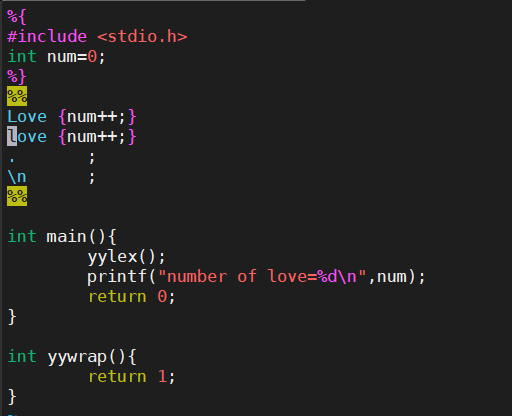
\includegraphics[width=3.45in]{1.png}
\label{picture}
\end{figure}

love.txt 속에 들어있는 love,Love를 구하는 문제 였다. 정의절에 num으로 선언해둔뒤 규칙절에서 Love 패턴이나 love패턴을 만나면 num을 1씩 증가해주는 연산을 하기ove.txt 속에 들어있는 love,Love를 구하는 문제 였다. 정의절에 num으로 선언해둔뒤 규칙절에서 Love 패턴이나 love패턴을 만나면 num을 1씩 증가해주는 연산을 하기로  한다. 

% ====================
% # hw2_2 #
% ====================

\section{hw2_2}

\begin{figure}[ht!] %!t
\centering
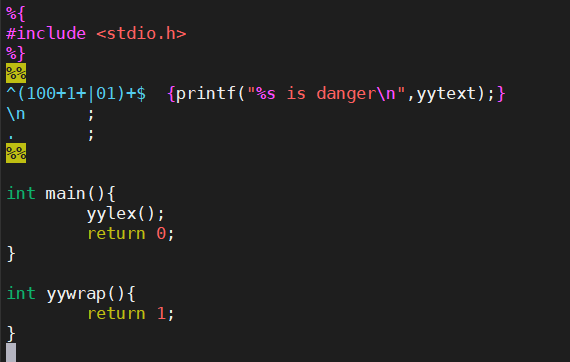
\includegraphics[width=3.45in]{2.png}
\label{picture}
\end{figure}

지난 파이썬과제 6번을 lex코드로 작성하는 문제이다. (100~1~|01)~ 를 만나면is danger 을 출력하는 것으로 위의 1번 처럼 정의절에서 num과 같은 카운트를 담당하는 변수를 사용할 필요가 없다. \^과 \$로 문자의 시작과 끝을 지정해 주었다. M+는 M을 1회반복한다는 뜻으로 위의 (100~1~|01)~의 ~을 모두 +로 바꾸면 정규식 완성이다.

% ==========================
% # hw2_3 #
% ==========================

\section{hw2_3}

\begin{figure}[ht!] %!t
\centering
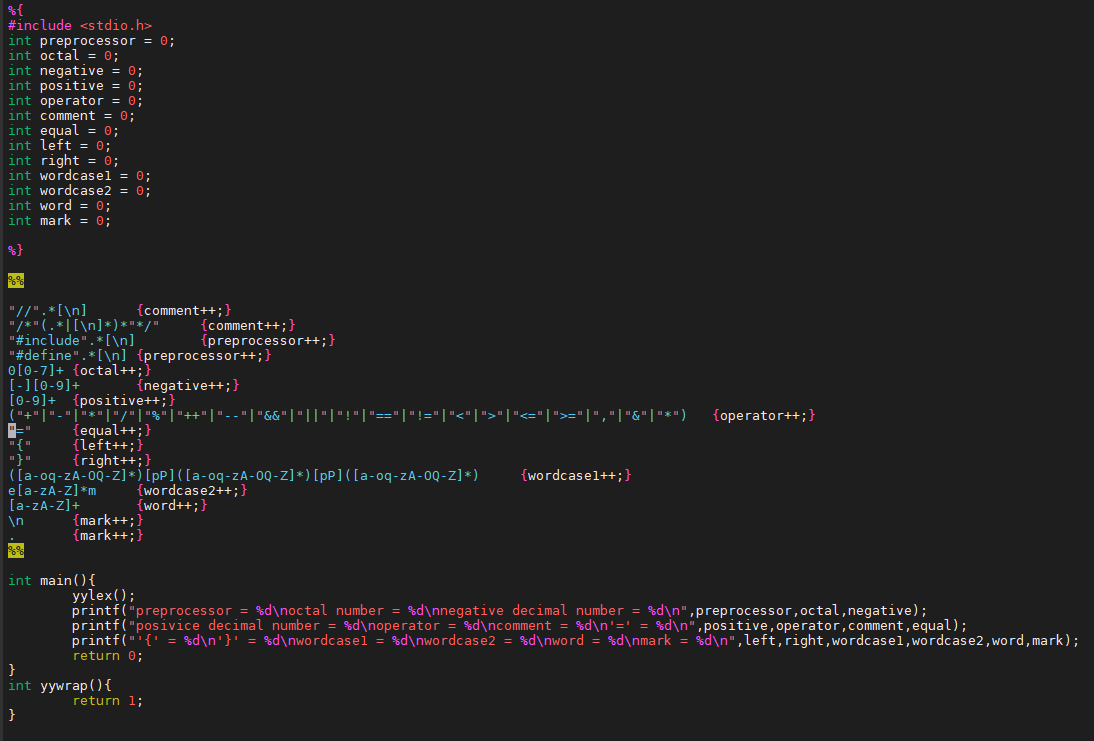
\includegraphics[width=3.4in]{3.png}
\label{bench}
\end{figure}
	test.c에 있는 문자,연산자 등 13가지에 대해 출력하는 코드를 작성하는 문제이다. \\
	정의절에서 카운트해야할 변수들에 대해서 우선 0으로 초기화 해주었다. \\
	그 후 규칙절에서는 첫번째로 주석에 대한 정규식을 먼저 작성하였다. 왜냐하면 주석안에 있는 문제들에 대해서는 count를 하지 않기 때문이다. //의 주석에 대해서는 // 뒤에 나오는 문자들과 개행문자를 함께 무시해 주도록 하였다. \\ /**/ 주석에 대해서는 /* 뒤로나오는 여러 문자들과 여러 개행문자들을 모두 무시해 주기 위해서 뒤에도 * 붙여주었다. 두번째부터는 출력값 차례대로 규칙절을 세워 주었다. 전처리문 두가지에 대해서도 //주석문과 같이 뒤에 나오는 문자들과 개행문자들을 무시해 주었다. \\
    c언어에서는 8진수를 0X로 표현한다. 그러므로 0과 0~7까지의 수를 합한 0[0-7]+로 표현하였다. \\
    양의 정수와 음의 정수는 0~9의 수들이 1회이상 반복되어 생기므로 [0-9]+와 [-][0-9]+로 표현하였다.\\
    여러 명령어와 등호, 중괄호는 쉽게 표현할 수 있었다.\\
    p가 두번이 들어간 문자는 p/P를 제외한 알파벳이나 공백 + p/P + p/P를 제외한 알파벳이나 공백 + p/P +  p/P를 제외한 알파벳이나 공백으로 표현하였다.\\
    e로 시작하고 m으로 끝나는 문자는 e+ 알파벳 0회이상 반복+m 으로 표현하였다.\\
    남은 문자들은 [a-zA-Z]의 1회이상 반복으로 표현하였으며 개행과 . 으로 mark의 수를 카운트해주었다.\\


\end{document}